\documentclass[12pt,a4paper]{article}
\usepackage[utf8]{inputenc}
\usepackage[portuguese]{babel}
\usepackage[T1]{fontenc}
\usepackage{mathtools}
\usepackage{amsfonts}
\usepackage{amssymb}
\usepackage{natbib}

\usepackage{fancyhdr}


\pagestyle{fancy}


% Permite juntar arquivos que tenham \documentclass
\usepackage{standalone}

% Table of Contents
\usepackage{hyperref}
\hypersetup{
    colorlinks,
    citecolor=black,
    filecolor=black,
    linkcolor=black,
    urlcolor=black
}

% Avaliar somente sintaxe dos arquivos.
%\usepackage{syntonly}
%\syntaxonly % Comente para somente avaliar sintaxe.



% Quadrado de final de prova.
\newcommand{\qed}{\hfill $\blacksquare$}


\newtheorem{lema}{Lema}[section]

\renewcommand{\baselinestretch}{1.5}

\everymath{\displaystyle}

\author{Sérgio Rodrigues}
\title{FGV\\ Álgebra Linear e Aplicações\\ Lista 1}
\begin{document}
\maketitle

%\tableofcontents

\newpage
\section*{Exercício 1}
É verdade que existe um polinômio de grau 3 que passa pelos pontos $ P_1= (0,1) $, $ P_2= (1,0) $, $ P_3= (2,-1) $, $ P_4= (3,2) $? Como encontrá-lo? Mostre que este problema é equivalente a resolver um sistema linear. Use um pacote computacional para resolver o sistema e para desenhar um gráfico com os pontos
$ P_i $ e este polinômio interpolador.

\underline{Interpolação Polinomial}

Sejam n+1 pontos dados por $ (x_i, f_i) $, $ 0 \leq i \leq n $. Então existe um único polinômio de grau $ n $ que passa por estes pontos: 

$ P_n(x) = a_0 + a_1x+ a_2x^2 + ... + a_nx^n = \sum_{i=0}^{n} a_ix^i$, sendo $ a_i \in \mathbb{R} $.

Dado $ P_n(x_i) = f_i$, é equivalente ao sistema:

\begin{align*}
	\begin{cases}
		a_0 + a_1x_0+ a_2x_0^2 + ... + a_nx_0^n = f_0\\
		a_0 + a_1x_1+ a_2x_1^2 + ... + a_nx_1^n = f_1\\
		\vdots\\
		a_0 + a_1x_n+ a_2x_n^2 + ... + a_nx_n^n = f_n\\
	\end{cases}
\end{align*}

Que pode ser representado como:

\begin{align*}
\begin{bmatrix}
1 & x_0 & x_0^2 & ... & x_0^n \\ 
1 & x_1 & x_1^2 & ... & x_1^n \\ 
\vdots & \vdots & \vdots & \vdots &  \vdots\\ 
1 & x_n & x_n^2 & ... & x_n^n
\end{bmatrix} 
\cdot
\begin{bmatrix}
a_0\\
a_1\\
\vdots\\
a_n
\end{bmatrix}
=
\begin{bmatrix}
f_0\\
f_1\\
\vdots\\
f_n
\end{bmatrix}
\end{align*}

Então, conforme o enunciado, temos:

\begin{align*}
\begin{bmatrix}
1 & 0 & 0^2 & 0^3  \\ 
1 & 1 & 1^2 & 1^3 \\ 
1 & 2 & 2^2 & 2^3 \\ 
1 & 3 & 3^2 & 3^3
\end{bmatrix} 
\cdot
\begin{bmatrix}
a_0\\
a_1\\
\vdots\\
a_n
\end{bmatrix}
=
\begin{bmatrix}
1\\
0\\
-1\\
2
\end{bmatrix}
\end{align*}

Utilizando o software R, temos que a solução é $ a_0 = 1$, $ a_1=1/3 $, $a_2=-2  $ e $ a_3=2/3 $, dando o polinômio $ P = 1 + x/3 -2x^2 + 2x^3/3  $:


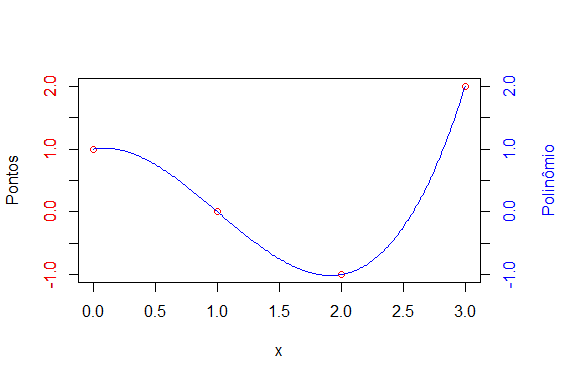
\includegraphics[width=1\linewidth]{./ex1}


Script em R:
\begin{verbatim}
# Exercicio 1.
# Criar matriz com repetição: http://www.ats.ucla.edu/stat/r/library/matrix_alg.htm
# Opções de plot http://www.statmethods.net/advgraphs/axes.html

# Construir matrizes A e b.
l = c(0,1,2,3)
A = c()
for( i in 1:length(l)){  
  A = cbind(A,l^(i-1))
}
b = c(1,0,-1,2)

# Solução do sistema linear Ax=b
a = solve(A,b) 



X = cbind(A[,2],b) # Pontos originais.

x=seq(0,3,0.01)

Pn = a[1]+a[2]*x+a[3]*x^2+a[4]*x^3
# create extra margin room on the right for an axis 
par(mar=c(5, 4, 4, 5) + 0.1)
plot(X,type='p',col='red',ylab='')
lines(x,Pn,type='l',col='blue')

# Eixo esquerdo.
axis(2,col.axis='red')

# Eixo direito.
axis(4,col.axis='blue',las=0)

# add a title for the right axis 
mtext("Polinômio", side=4, line=3, cex.lab=1, las=0, col="blue")

title( ylab='Pontos', xlab='x')
\end{verbatim}
\qed


\newpage
\section*{Exercício 2}
Seja $A = \begin{bmatrix}
1 & 0 & 1 \\ 
2 & 1 & 1 \\ 
3 & 1 & 2 \\ 
3 & 2 & 1
\end{bmatrix} $. Use eliminação gaussiana para verificar se o sistema $ A \cdot x = b $, onde $ b =[1,2,3,1]^T $, tem solução.

Eliminação gaussiana:

\begin{align*}G=
\begin{bmatrix}
1 & 0 & 1 & 1\\ 
2 & 1 & 1 & 2\\ 
3 & 1 & 2 & 3\\ 
3 & 2 & 1 &1
\end{bmatrix}
\xrightarrow[]{[1]}
\begin{bmatrix}
1 & 0 & 1 & 1\\ 
0 & 1 & -1 & 0\\ 
0 & 1 & -1 & 0\\ 
0 & 1 & -1 &-1
\end{bmatrix}
\end{align*}

[1]: $ L_2 \leftarrow L_2 - 2L_1 $; $ L_3 \leftarrow L_3 - 3L_1 $; $ L_4 \leftarrow (L_4 - 3L_1)/2 $

Temos que na matriz G as entradas $ G_{3,4} $ e $ G_{4,4} $ são diferentes para coeficientes $ G_{3,m} $ e $ G_{4,n} $ iguais, $ m $ e $ n $ $ \in \{1,2,3\} $. O que mostra que o sistema não tem solução.
\qed


\newpage
\section*{Exercício 3}
\subsection*{Strang, conjunto 1.3 - 15 - Inlgês}
If rows 1 and 2 are the same, how far can you get with elimination (allowing row exchange)? 
\begin{align*}
\begin{bmatrix}
2 & -1 & 1 & 0\\
2 & -1 & 1 & 0\\
4 & 1  & 1 & 2
\end{bmatrix}
\xrightarrow{[1]}
\begin{bmatrix}
2 & -1 & 1 & 0\\
0 & 3  & -1 & 2\\
0 & 0 & 0 & 0\\
\end{bmatrix}
\end{align*}
$ [1]: L_2 \leftrightarrow L_3; L_2\leftarrow L_2-2L_1; L_3 \leftarrow L_3-L_1$

Temos que a variável $ z $ é livre. Façamos $ z=t $, então:
\begin{align*}
0x +0y + z &= t\\
0x + 3y -t &=2 \Rightarrow y = \dfrac{2+t}{3} \\
2x -y +t &= 0 \Rightarrow x = \dfrac{1-t}{3}
\end{align*}

O sistema tem infinitas soluções do tipo $ (\dfrac{1-t}{3}, \dfrac{2+t}{3}, t ) $.\\


If columns 1 and 2 are the same, which pivot is missing?
\begin{align*}
\begin{bmatrix}
2 & 2 & 1  & 0\\
4 & 4 & 1  & 0\\
6 & 6 & 1  & 2
\end{bmatrix}
\xrightarrow{[1]}
\begin{bmatrix}
2 & 2 & 1  & 0\\
0 & 0 & -2  & 2\\
0 & 0 & -1  & 0
\end{bmatrix}
\end{align*}
$ [1]: L_3 \leftrightarrow L_2; L_2 \leftarrow L_2 - 3L_1; L_3 \leftarrow L_3 - 2L_1 $.

Se as colunas 1 e 2 são iguais, mesmo com a troca de linhas, indicada acima o pivot ausente é o da variável $ y $, respectivo à coluna que repetiu. Entretanto, este exemplo apresenta uma contradição nas linhas 2 e 3, que o torna sem solução.
\qed

\subsection*{Strang, conjunto 1.3 - 15 - Português}
É impossivel um sistema de equações lineares ter exatamente duas soluções. Explique porquê.

A solução de um sistema linear é um ponto no espaço $ n $-dimensional comum a todos os hiper planos definidos pelas $ n $ equações. Assim, existe o vetor $ = (x_1,x_2,\cdots,x_n) $ que satisfaz $ A\cdot x = b $. Se admitirmos que exista outro vetor $ y $ tal que $ A \cdot y = b $, então temos que $ A\cdot x = A \cdot y $, o que leva à conclusao de que $ x = y $. 
\qed

(a) Se $ (x,y,z) $ e $ (X,Y,Z) $ são duas soluções, qual seria outra?

Qualquer ponto na reta onde passa os pontos do enunciado.
\qed

(b) Se 25 planos se encontram em 2 pontos, onde mais eles se encontram?




\subsection*{Strang, conjunto 1.3 - 22 - Inglês}
 Apply elimination and back-substitution to solve
\begin{align*}
2u + 3v + 0w =  0\\
4u + 5v + w = 3\\
2u - v - 3w = 5
\end{align*}
What are the pivots? List the three operations in which a multiple of one row is subtracted from another. 
\begin{align*}
\begin{bmatrix}
2 &  3 &  0 &   0\\
4 &  5 &  1 &  3\\
2 & -1  & - 3 &  5
\end{bmatrix}
\xrightarrow{[1]}
\begin{bmatrix}
2 &  3 &  0 &   0\\
0 &  1 &  -1 &  -3\\
0 & 4  & 3 &  -5
\end{bmatrix}
\xrightarrow{[2]}
\begin{bmatrix}
2 &  3 &  0 &   0\\
0 &  1 &  -1 &  -3\\
0 & 0  & 1 &  1
\end{bmatrix}
\xrightarrow{[3]}
\end{align*}
\begin{align*}
\xrightarrow{[3]}
\begin{bmatrix}
1 &  0 &  0 &   3\\
0 &  1 &  0 &  -2\\
0 & 0  & 1 &  1
\end{bmatrix}
\Rightarrow
[u,v,w]^T = [3, -2, 1]^T
\end{align*}
$ [1] : L_2 \leftarrow L_2 - 2L_1; L_3 \leftarrow L_3 - L_1; L_2 \leftarrow -L_2; L_3 \leftarrow -L_3 $\\
$ [2] : L_3 \leftarrow L_3 - 4L_2; L_3 \leftarrow L_3/7 $\\
$ [3] : L_2 \leftarrow L_2 + L_3; L_1 \leftarrow L_1 - 3L_2; L_1 \leftarrow L_1/2.$
\qed

\subsection*{Strang, conjunto 1.3 - 22 - Português}
Encontre os pivôts e soluções:

\begin{align*}
\begin{bmatrix}
2 & 1 & 0 & 0 & 0\\
1 & 2 & 1 & 0 & 0\\
0 & 1 & 2 & 1 & 0\\
0 & 0 & 1 & 2 & 5
\end{bmatrix}
\xrightarrow{[1]}
\begin{bmatrix}
\underline{2} & 1 & 0 & 0 & 0\\
0 & \underline{3} & 2 & 0 & 0\\
0 & 0 & \underline{4} & 3 & 0\\
0 & 0 & 0 & \underline{5} & 20
\end{bmatrix}
\xrightarrow{[2]}
\begin{bmatrix}
1 & 0 & 0 & 0 & -1\\
0 & 1 & 0 & 0 & 2\\
0 & 0 & 1 & 0 & -3\\
0 & 0 & 0 & 1 & 4
\end{bmatrix}
\end{align*}
\qed

\newpage
\section*{Exercicio 4}
\subsection*{Strang, conjunto 1.4 - exercício 8}
Do these subroutines multiply \textit{Ax b y rows or columns}? Start with $ B(I) = 0 $:


DO 10 I = 1, N\\
DO 10 J = 1, N\\
10 B(I) = B(I) + A(I,J) * X(J)
\\

DO 10 J = 1, N\\
DO 10 I = 1, N\\
10 B(I) = B(I) + A(I,J) * X(J)

The outputs $ Bx = Ax $ are the same. The second code is slightly more efficient in
FORTRAN and much more efficient on a vector machine (the first changes single
entries B(I), the second can update whole vectors).

\subsection*{Strang, conjunto 1.4 - exercício 9 - Inglês}
 If the entries of $ A $ are $ a_{ij} $, use subscript notation to write

(a) the first pivot.

$ a_{1,1} $
\qed
\\

(b) the multiplier $ l_{i1} $ of row 1 to be subtracted from row $ i $.

$ a_{i,1} - l_{i,1}a_{1,1} = 0 \Rightarrow l_{i,1} = \dfrac{a_{i,1}}{a_{1,1}} $
\qed
\\

(c) the new entry that replaces $ a_{ij} $ after that subtraction.

$ a_{i,j} \leftarrow a_{i,j} - \dfrac{a_{i,1}}{a_{1,1}}a_{1,j} $
\qed
\\

(d) the second pivot.

$ a_{2,2} $
\qed


\subsection*{Strang, conjunto 1.4 - exercício 9 - Português}
O produto de duas matrizes triangulares inferiores é também triangular inferior. Confirme com um exemplo 3x3 e explique com a lei das multiplicações de matrizes.

Explicação:

Seja $ C_{m\times n} = A_{m \times p}\cdot B_{p \times n} $.
\\

Para $ \forall i,j $, $ 1\leq i \leq m $ e $ 1\leq j \leq n $: 
$
c_{i,j} = \sum_{k=1}^{p} (a_{i,k}\cdot b_{k,j})
$
\\

Mas $ A,B $ são triangulares inferiores, então $ \forall j>i, a_{i,j}=0 $ e $ b_{i,j} = 0 $.
\\

Portanto $ c_{i,j} = \begin{cases}
\sum_{k=1}^{p} (a_{i,k}\cdot b_{k,j})&\text{, se } j\leq i\\
0, &\text{, se j>i }
\end{cases} $

Exemplo:

\begin{align*}
\begin{bmatrix}
13 & 0 & 0 \\ 
26 & 20 & 0 \\ 
11 & 19 & 1 \\ 
\end{bmatrix}
\cdot
\begin{bmatrix}
22 & 0 & 0 \\ 
15 & 24 & 0 \\ 
5 & 7 & 1 \\ 
\end{bmatrix}
\cdot
\begin{bmatrix}
286 & 0 & 0 \\ 
872 & 480 & 0 \\ 
532 & 463 & 1 \\ 
\end{bmatrix}
\end{align*}
\qed

\newpage
\section*{Exercício 5}
(Trefethen) Considere a matriz B de dimensões 4x4. Sobre ela são aplicadas as seguintes operações:

(a) Multiplicar a coluna 1 por 2

(b) Dividir a linha 1 por 3

(c) Adicionar a linha 3 à linha 1

(d) Trocar a coluna 1 com a coluna 4 de lugar

(e) Subtrair a linha 2 das demais linhas

(f) Substituir a coluna 4 pela coluna 3

(g) eliminar a coluna 1 (portanto o número de colunas é reduzido para 3)

i.Escreva o resultado como produto de 8 matrizes

\begin{align*}
e \cdot c \cdot b \cdot B \cdot a \cdot d \cdot f \cdot g
\end{align*}
\begin{align*}
\begin{scriptsize}
\begin{bmatrix} %e
1 & -1 & 0 & 0 \\ 
  0 & 1 & 0 & 0 \\ 
  0 & -1 & 1 & 0 \\ 
  0 & -1 & 0 & 1 
\end{bmatrix}
\begin{bmatrix} %c
1 & 0 & 1 & 0 \\ 
0 & 1 & 0 & 0 \\ 
0 & 0 & 1 & 0 \\ 
0 & 0 & 0 & 1
\end{bmatrix}
\begin{bmatrix} %b
0.33 & 0 & 0 & 0 \\ 
0 & 1 & 0 & 0 \\ 
0 & 0 & 1 & 0 \\
0 & 0 & 0 & 1 
\end{bmatrix}
B
\begin{bmatrix} %a
2 & 0 & 0 & 0 \\ 
0 & 1 & 0 & 0 \\ 
0 & 0 & 1 & 0 \\ 
0 & 0 & 0 & 1
\end{bmatrix}
\begin{bmatrix} %d
0 & 0 & 0 & 1 \\ 
0 & 1 & 0 & 0 \\ 
0 & 0 & 1 & 0 \\ 
1 & 0 & 0 & 0
\end{bmatrix}
\begin{bmatrix} %f
1 & 0 & 0 & 0 \\ 
  0 & 1 & 0 & 0 \\ 
  0 & 0 & 0 & 1 \\ 
  0 & 0 & 1 & 0 
\end{bmatrix}
\begin{bmatrix} %g
1 & 0 & 0 & 0 \\ 
0 & 1 & 0 & 0 \\ 
0 & 0 & 0 & 1 \\ 
0 & 0 & 1 & 0 
\end{bmatrix}
\end{scriptsize}
\end{align*}
\qed
\\

ii. Escreva o resultado novamente como um produto A · B · C (mesmo B do enunciado) de três matrizes.

\begin{align*}
\begin{bmatrix}{}
0.33 & -1 & 1 & 0 \\ 
0 & 1 & 0 & 0 \\ 
0 & -1 & 1 & 0 \\ 
0 & -1 & 0 & 1 \\ 
\end{bmatrix}
B
\begin{bmatrix}{}
0 & 2 & 0 \\ 
1 & 0 & 0 \\ 
0 & 0 & 1 \\ 
0 & 0 & 0 \\ 
\end{bmatrix}
\end{align*}
\qed 

\newpage
\section*{Exercício 6}
 Monte um programa que tem como entrada uma matriz $ L_{n,n}  $triangular inferior e um vetor $ b_{n,1} $ e
devolve um vetor $ x_{n,1} $ que é a solução de $ L\cdot x = b $. O algoritmo implementado deve ter complexidade
$ O(n^2) $.

Script em R:

\begin{verbatim}
# Retorna a matriz triangular inferior de uma matriz como parâmetro.
lowtri <- function(matr) {
  lt <- matrix(0, nrow=nrow(matr), ncol=ncol(matr))
  for (i in 1:nrow(matr)) {
    for (j in 1:i) {
      lt[i,j] <- matr[i,j]
    }
  }
  return(lt)
}

# INÍCIO DO PROGRAMA.
# Determina tamanho da matriz n*n.
n = 10

# Define matriz triangular inferior com valores aleatórios.
L = lowtri(matrix(sample(1:n^2),c(n,n)))

# Define vetor aleatório.
b = sample(1:n,n)

# Concatena matrizes para eliminação gaussiana.
matriz = cbind(L,b)

# Resolve com eliminação gaussiana.
n = nrow(matriz)
for(j in 1:(n-1)){
  matriz[j,] = matriz[j,]/matriz[j,j]
  for(i in (j+1):n){
    matriz[i,] = matriz[i,]-(matriz[i,j]*matriz[j,])
  }
}
matriz[n,] = matriz[n,] /matriz[n,n] 

# Imprime fim da eliminação.
matriz
\end{verbatim}
\qed


\newpage
\section*{Exercicio 7}
Estime a complexidade do algoritmo de solução de sistemas lineares do pacote computacional de sua
preferência: registre os tempos que o pacote levou para resolver sistemas aleatórios $ n \cdot n $, com $ n =
16,32,64,128,256,512,1024,2048 $. Faça um gráfico do log do número de colunas contra o log dos tempos
registrados. O algoritmo do pacote tem complexidade inferior a $ O(n^3) $?
\\

Ao executar o script abaixo obtemos o seguinte resultado:

\begin{tabular}{|c|c|c|c|c|c|c|c|c|c|c|}
\hline log2(n) & 4 & 5 & 6 & 7 & 8 & 9 & 10 & 11 & 12 & 13 \\ 
\hline log2(t) & 0 & 0 & 0 & 0 & 0.03 & 0.13 & 0.95 & 6.95 & 55.53 & 446.83\\ 
\hline 
\end{tabular} 

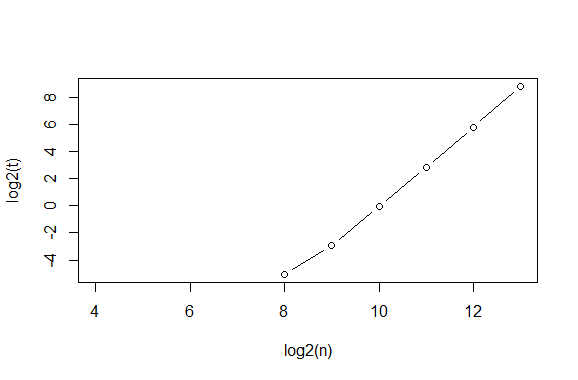
\includegraphics[width=0.8\linewidth]{./ex7}

Script:

\begin{verbatim}
# Retorna a matriz triangular inferior de uma matriz como parâmetro.
random_matrix <- function(n) {
  matrix(sample(1:n^2),c(n,n))
}


# Resolve um sistema aleatorio A.x=b de tamanho n onde A é nxn e b é 1xn.
solve_random <- function(n){
  A = random_matrix(n)
  b = sample(1:n,n)
  
  return(system.time(solve(A,b)))
}



# INÍCIO DO PROGRAMA.
n <- 2^c(5:13)
t = sapply(n, function(n) solve_random(n))
t = t[3,]
plot(log2(n),log2(t),type='b' )

# Regressao linear para determinar inclinação.
# Fonte: http://www.cyclismo.org/tutorial/R/linearLeastSquares.html
fit = lm(t ~ n)
On = fit$coefficients[[2]] # Inclinação é a complexidade.

print(On)
\end{verbatim}
\qed


\end{document}